\section{Komparator LM311}
Zbudowano układ wykorzystując płytkę UA-1 oraz komparator napięcia LM311 (Rys. \ref{sh1}).
Mając na uwadze to aby napięcie chwilowe nie przekraczało napięcia zasilającego, dobrano amplitudę napięcia sinusoidalnego generatora \(U=5V\).
Następnie za pomocą rezystora nastawnego na płytce UA-1 podawano na wejście nieodwracające napięcie z zakresu międzyszczytowego napięcia generatora.

Uzyskano w ten sposób falę prostokątną na wyjściu komparatora, o współczynniku wypełnienia zależnym od napięcia podanego przez potencjometr.
Pomiar napięcia wyjściowego wykonano dla częstotliwości: \(10kHz\), \(50kHz\), \(100kHz\). Zaobserwowano wzrost czasu narastania sygnału wyjściowego wraz z ze wzrostem częstotliwości sygnału wejściowego z generatora funkcyjnego.

\begin{figure}[H]
    \centering
    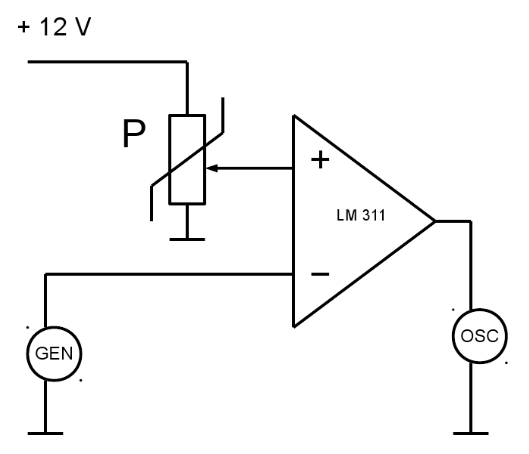
\includegraphics[width=7.5cm]{include/1/1.png}
    \caption{Schemat zbudowanego układu.}
    \label{sh1}
\end{figure}

\begin{figure}[H]
    \centering
    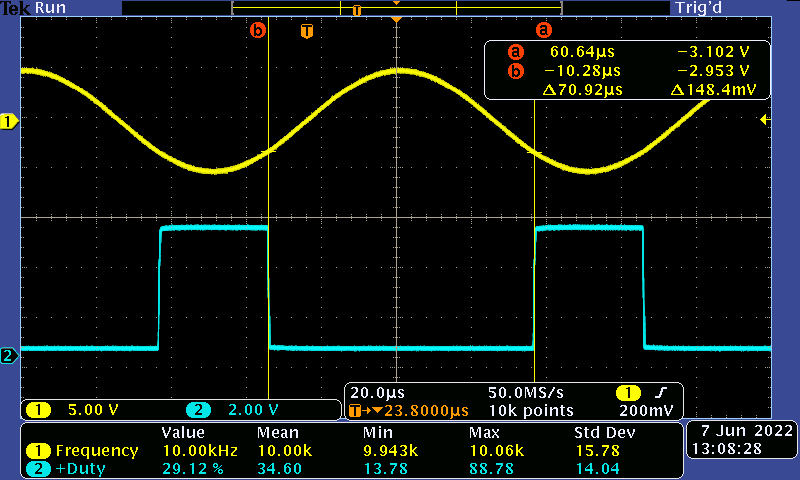
\includegraphics[width=\textwidth]{include/1/2.png}
    \caption{Odpowiedź układu dla napięcia na wejściu nieodwracającym \(-3.067V\).}
\end{figure}

\begin{figure}[H]
    \centering
    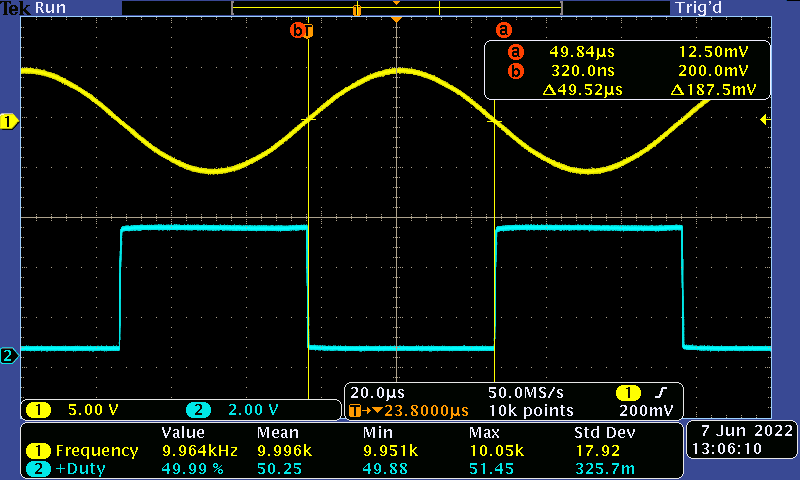
\includegraphics[width=\textwidth]{include/1/3.png}
    \caption{Odpowiedź układu dla napięcia na wejściu nieodwracającym \(0.011V\).}
\end{figure}

\begin{figure}[H]
    \centering
    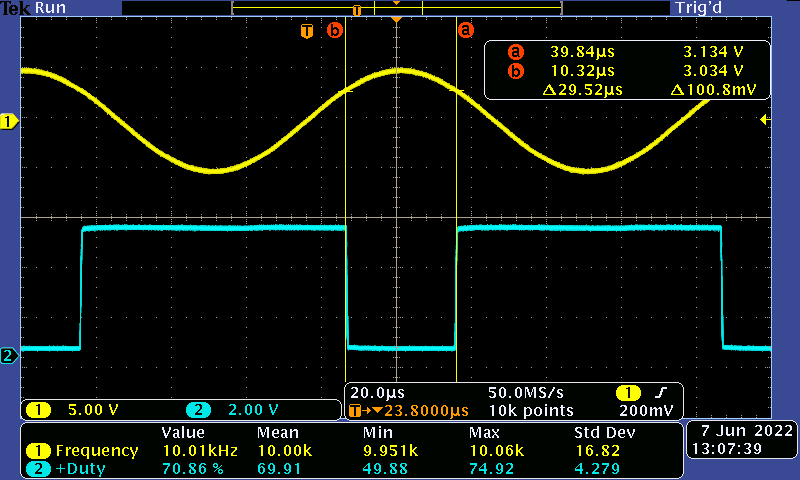
\includegraphics[width=\textwidth]{include/1/4.png}
    \caption{Odpowiedź układu dla napięcia na wejściu nieodwracającym \(3.093V\).}
\end{figure}
